\documentclass[11pt]{article}

\usepackage[utf8]{inputenc}
\usepackage[T1]{fontenc}
\usepackage{geometry}
\usepackage{amsmath,amssymb,amsthm}
\usepackage{booktabs}
\usepackage{graphicx}
\usepackage{array}
\usepackage{microtype}
\usepackage[hidelinks]{hyperref}

\geometry{margin=1in}

% One number, one place. Every number in the paper comes from here, and every
% macro here comes from a counted pass over the corpus or over wiki/sources.
% Regenerate the corpus counts with tools/corpus-counts.sh.

% Corpus, counted 2026-08-22.
\newcommand{\NumPapers}{206}          % PDFs in raw/
\newcommand{\NumSources}{200}         % source pages in wiki/sources/
\newcommand{\NumConcepts}{83}
\newcommand{\NumEntities}{116}

% Mapping results. Filled by the Part V generator; do not hand-edit.
\newcommand{\NumUnstated}{37}          % works stating no budget for any party
\newcommand{\NumPriced}{163}         % works bounding at least one party

% --- Numbers used in Part I. Each traces to a wiki source page that was
% --- verified against the primary PDF in the 2026-08-22 audit.
% mia-from-first-principles, blind-baselines-beat-mia, sok-mia-llms-rushing-nowhere,
% do-mias-work-on-llms
\newcommand{\MIAnewMethods}{ten}      % new MIA methods proposed in 2024 alone
\newcommand{\MIAblindSets}{eight}     % published MI evaluation datasets beaten by blind baselines
\newcommand{\MIAwikiLo}{0.988}        % bag-of-words AUC on WikiMIA, low
\newcommand{\MIAwikiHi}{0.994}        % bag-of-words AUC on WikiMIA, high
\newcommand{\MIAmimirAUC}{0.6}        % ceiling on MIMIR outside GitHub
% obfuscated-gradients
\newcommand{\OGpopulation}{nine}      % non-certified ICLR 2018 defences claiming white-box robustness
\newcommand{\OGobfuscated}{seven}     % of those relying on obfuscated gradients
\newcommand{\OGbrokenFull}{six}
\newcommand{\OGbrokenPart}{one}
% adaptive-attacks-defenses
\newcommand{\AAdefences}{thirteen}
% dos-and-donts-ml-security
\newcommand{\DDpapers}{30}            % papers from CCS, S&P, USENIX Security, NDSS
\newcommand{\DDpitfalls}{ten}
\newcommand{\DDminPitfalls}{three}    % pitfalls affecting every one of the 30
% sok-black-box-attack-pitfalls
\newcommand{\BBattacks}{164}
\newcommand{\BBmajorVenue}{102}
\newcommand{\BBrerun}{eleven}          % transfer attacks re-run under one time budget
\newcommand{\BBminutes}{30}            % minutes per batch in that re-run

% Corpus breadth, counted over wiki/sources/ front-matter tags on 2026-08-22.
\newcommand{\NumMIApages}{21}         % source pages mentioning membership inference
\newcommand{\NumMIAfamily}{12}        % works whose attack family is membership

% --- Findings read off the classification tables. Counted by tools/collect-cls.py
% --- over notes/classification.tsv on 2026-08-22. Regenerate before submission.
\newcommand{\NumAttackWorks}{103}     % works carrying an attack family
\newcommand{\NumTheoryWorks}{97}      % works carrying none
\newcommand{\NumPhaseAccessCells}{19} % populated cells of 32 in phase x access
\newcommand{\NumPartyUnitCells}{25}   % populated cells of 75 in party x unit
\newcommand{\AttackAccessNamed}{72}   % attack works naming an access level
\newcommand{\AttackPostHoc}{34}       % of those, attacking a released model
\newcommand{\AttackTestTime}{25}      % of those, at test time
\newcommand{\AttackTrainTime}{12}     % of those, at training time
\newcommand{\AttackQueriesAttacker}{9} % attack works whose adversary is bounded in queries
\newcommand{\AttackSamplesAttacker}{2} % attack works whose adversary is bounded in samples
\newcommand{\NumExponent}{20}         % works stating an exponent in one party's own resource
\newcommand{\AttackUnbound}{27}       % attack works bounding no party
\newcommand{\TheoryUnbound}{10}        % non-attack works bounding no party
\newcommand{\AttackBudget}{36}        % attack works whose bound is a budget
\newcommand{\AttackUnstated}{28}      % attack works stating no tightness
\newcommand{\AttackPoly}{17}
\newcommand{\AttackMeasured}{12}
\newcommand{\AttackClass}{4}
\newcommand{\AttackPerturb}{20}       % attack works bounded by a perturbation radius
\newcommand{\AttackCorrupt}{5}        % attack works bounded by a corruption fraction

% --- Sparse-parity experiment, exp/survey/experiments/, run 2026-08-22.
% Config: k=3, 2-layer ReLU width 100, batch 128, lr 0.01, fresh batches,
% threshold 0.90 test accuracy, 8 seeds per dimension, d in {20,30,40,50,60}.
% Source: canonical_b128.json (regenerate: sparse_parity.py, seeds fixed).
\newcommand{\ParityK}{3}
\newcommand{\ParitySlope}{2.02}       % fitted log-log exponent of median steps vs d
\newcommand{\ParitySeeds}{8}
\newcommand{\ParityDims}{20 to 60}
\newcommand{\ParitySolved}{40 of 40}  % runs reaching threshold within budget
\newcommand{\ParityMedLoD}{1025}      % median steps at d=20
\newcommand{\ParityMedHiD}{9337.5}    % median steps at d=60 (mean of 4th and 5th of 8)
% Probe regime: batch 8, otherwise width 512 lr 0.1; steps at d=30 vs cap at d=60.
\newcommand{\ProbeMedThirty}{6940}
\newcommand{\ProbeCap}{300000}
\newcommand{\ParityThresh}{90\%}

% --- The near-miss set: works whose treatment of a resource does not match how
% --- tightly they state it. Counted 2026-08-27.
\newcommand{\AssessedPredictable}{90}   % per cent predictable from tightness alone
\newcommand{\NearMiss}{19}              % works where the two disagree
\newcommand{\NearMissA}{10}             % definitional bound, not treated as the object
\newcommand{\NearMissB}{8}              % measured cost, treated deliberately
\newcommand{\NearMissC}{1}              % quantity present, no tightness at all

% --- Baseline column, countable after the re-pass of 2026-08-27.
\newcommand{\BaselineCrit}{50}
\newcommand{\BaselineStated}{29}
\newcommand{\BaselineAbsent}{21}
\newcommand{\BaselineNA}{133}
\newcommand{\BaselineChanged}{31}
\newcommand{\NumRelative}{18}
\newcommand{\NumRelativeAttack}{6}
\newcommand{\NumFlops}{5}
\newcommand{\AttackTimeAttacker}{17}
\newcommand{\ThmAttack}{71}
\newcommand{\ThmOther}{87}
\newcommand{\ThmAttackUnbound}{12}
\newcommand{\ThmOtherUnbound}{6}

% --- Added by check-numbers.py --write; computed from the classification.
\newcommand{\RateAttack}{26}
\newcommand{\RateOther}{10}
\newcommand{\RatioUnbound}{2.5}
\newcommand{\DiffLo}{5.5}
\newcommand{\DiffHi}{26.3}
\newcommand{\ThmRatio}{2.5}
\newcommand{\ThmDiffLo}{$-0.2$}
\newcommand{\ThmDiffHi}{20.2}
\newcommand{\NumScaling}{10}
\newcommand{\PhaseAccessTopFive}{62}
\newcommand{\PartyUnitTopFive}{78}
\newcommand{\NearMissAdv}{9}
\newcommand{\NearMissTrain}{5}
\newcommand{\NearMissCap}{5}
\newcommand{\AttackerTimeCirc}{34}
\newcommand{\AttackerCapability}{25}
\newcommand{\AttackerPerturbAll}{20}
\newcommand{\AttackerCorruptAll}{5}
\newcommand{\AttackerMemory}{4}
\newcommand{\LearnerBound}{65}
\newcommand{\LearnerTime}{21}
\newcommand{\LearnerSamples}{17}
\newcommand{\LearnerClass}{16}
\newcommand{\LearnerFlops}{5}
\newcommand{\LearnerOther}{6}
\newcommand{\AuditorBound}{10}
\newcommand{\MechanismBound}{7}
\newcommand{\QuoteOnFile}{172}
\newcommand{\QuoteAbsent}{28}
\newcommand{\QuoteHand}{0}

% --- Second quotation pass, tools/check-quotes.py bound through raw/SOURCES.md, run 2026-09-03.
\newcommand{\QuoteBound}{155}          % quotations verified in their own document
\newcommand{\QuoteUnbound}{5}        % not bound to a document by title, or no prose fragment


\theoremstyle{definition}
\newtheorem{definition}{Definition}
\newtheorem{example}{Example}
\theoremstyle{plain}
\newtheorem{proposition}{Proposition}
\newtheorem{fact}{Fact}
\theoremstyle{remark}
\newtheorem{openq}{Open}
\newtheorem{deferred}{Deferred}

\newcommand{\X}{\mathcal{X}}
\newcommand{\Y}{\mathcal{Y}}
\newcommand{\Lo}{\mathsf{L}}
\newcommand{\Rec}{\mathsf{R}}
\newcommand{\Tr}{\tau}
\newcommand{\View}{\mathsf{V}}
\newcommand{\A}{\mathcal{A}}
\newcommand{\C}{\mathcal{C}}
\newcommand{\D}{\mathcal{D}}
\newcommand{\cost}{\mathsf{cost}}
\newcommand{\steps}{\mathsf{steps}}

\title{The learning oracle\\
\large A self-contained statement of the framework, as agreed on 2026-08-22}
\author{}
\date{2026-08-22}

\begin{document}
\maketitle

\tableofcontents

\section{What this document is}

This document states, from nothing, the formal framework that the survey's
formalization section will rest on. It assumes the reader knows game-based
cryptography and machine learning, and assumes no prior exposure to the framework
itself. Every object is defined before it is used. Every claim is labelled as a
definition, a fact with a proof, a proposal, or an open question.

Two earlier artifacts exist. The extraction games in \texttt{games.tex} are one
instance of what is defined here, and Section~\ref{sec:map} says where they sit.
The survey's frame of four coordinates, access point, criterion, budget and
baseline, is recovered in Section~\ref{sec:games}, so nothing already written is
lost, and one coordinate, the budget, is replaced by something more specific.

\section{The problem the framework solves}
\label{sec:problem}

A security definition for a learned model has to say what the adversary may do.
For black-box access this is manageable: the adversary sends inputs and receives
outputs, and one counts the queries. For white-box access it is not. The adversary
holds the weights, and what it can learn from them depends on how training shaped
them. A definition that covers that case seems to require a theory of the training
map, the function from a corpus to a model. The map itself is public code that
anyone can run. What no theory describes is what the map produces, and whether
anything it produces can be obtained more cheaply than by running it.

Cryptography faced the same shape of problem with hash functions. No theory
describes what SHA-256 does to its input, so the random oracle model replaces the
hash function with an oracle that every party queries and no party can simulate,
and proves theorems relative to that oracle. The generic group model does the same
for group structure, and the Random Language Model of Brzuska and Couteau does it
for language membership \cite{BC22}. In each case the function is public, the hardness lies in reaching a
\emph{specified} output without paying the search or the walk, and the cost of an
attack is counted in oracle queries.

The framework below makes that move for learning. The one object we cannot describe
is the training map, so that is the one object the oracle idealizes. Inference is a
computable function, analysis of weights is ordinary computation, and data is
supplied by the game. The move has a precedent inside machine learning: the
generic learning model of Villa et al.\ is this idealization used for one theorem,
on the tension between a classifier's usefulness and membership privacy
\cite{VDKMR26}. What is new here is using it as the ambient model every game lives
in, and as the unit every party is priced in.

\section{Notation}
\label{sec:notation}

\begin{center}
\begin{tabular}{>{$}l<{$} l}
\toprule
\X, \Y & input space and output space of a model \\
D & a corpus, a finite multiset of labelled examples from $\X \times \Y$ \\
n & the security parameter, which scales the corpus, the model and the budgets \\
\Rec & a recipe, Definition~\ref{def:recipe} \\
w_t & the state of training after step $t$, a vector of weights \\
g_t & the gradient, or other per-step quantity, computed at step $t$ \\
\Tr & a training trace, Definition~\ref{def:trace} \\
\Lo & the learning oracle, Definitions~\ref{def:passive} and~\ref{def:interactive} \\
\View & a view, Definition~\ref{def:view} \\
\C, \A & the challenger and the adversary \\
\steps & the cost unit, one step of the recipe \\
\bottomrule
\end{tabular}
\end{center}

A \emph{party} is any algorithm in a game. The challenger runs the game. The
adversary tries to win it. Other named parties, an auditor or a second adversary,
appear where a game needs them. Everything is probabilistic polynomial time in $n$
unless a game says otherwise.

\section{Recipes and traces}
\label{sec:recipe}

The framework needs a name for a training procedure that is fixed and public but
whose behaviour on a given corpus we do not claim to understand.

\begin{definition}[Recipe]
\label{def:recipe}
A recipe $\Rec$ is a public description of a training procedure: an architecture,
a loss, an optimizer, a batch rule, an initialization rule, a step count $T$, and
any noise the procedure adds to its own computation. A recipe fixes a
\emph{step function} $S$ that carries the current state $w_{t-1}$ and a batch
$B_t$ to a per-step quantity $g_t$ and a new state $w_t$.
\end{definition}

A recipe is an object a paper would write in its experimental section. Stochastic
gradient descent on a named architecture with a named learning rate is a recipe.
Differentially private SGD, which clips and adds Gaussian noise to each gradient,
is a different recipe, and the noise is inside it.

\begin{definition}[Trace]
\label{def:trace}
The trace of running recipe $\Rec$ on corpus $D$ with coins $r$ is the sequence
\[
\Tr = \big(w_0;\; (B_1, g_1, w_1);\; (B_2, g_2, w_2);\; \dots;\; (B_T, g_T, w_T)\big),
\]
where $w_0$ is the initial state drawn by the initialization rule, $B_t$ the batch
drawn by the batch rule, and $(g_t, w_t) = S(w_{t-1}, B_t)$. The final model is
$w_T$. The \emph{length} of the trace is $T$.
\end{definition}

The trace is everything that happened during training, in order. A paper that
releases a model releases $w_T$. A paper on gradient leakage studies some of the
$g_t$. A proof-of-learning scheme asks a prover to exhibit a trace. These are all
views of one object, which is the reason the trace and not the model is the
oracle's output.

\section{The learning oracle, passive form}
\label{sec:passive}

\begin{definition}[Passive learning oracle]
\label{def:passive}
A game names a finite set of public recipes. The passive learning oracle
$\Lo_{\Rec}$ for a named recipe $\Rec$ is an oracle that, on input a corpus $D$,
draws fresh coins $r$, runs $\Rec$ on $D$ with $r$, and returns the trace $\Tr$.
Two calls on the same corpus return independent traces. Parties call the oracle
on the named recipes and do not author recipes of their own.
\end{definition}

\begin{definition}[Metered cost]
\label{def:cost}
The cost of a call is the computational work of executing the recipe on the
submitted corpus, in a fixed machine model, together with the size of that
corpus. Within one recipe, whose step function is fixed, the shorthand for that
work is the step count $T$, and this document prices calls in steps whenever the
recipe is clear from context. A party's oracle cost is the total over its calls.
A party also has its own running time, which is ordinary computation and is
accounted separately.
\end{definition}

Two restrictions inside these definitions carry weight, and each blocks a
concrete attack on the accounting itself. Recipes are named by the game rather
than submitted by parties, because an adversary permitted to author recipes
defeats the unit twice over. A wrapping recipe whose single step runs all $T$
steps of another recipe would collapse any step count to one, which is why cost
is defined as the work of the step function and steps are only a shorthand. A
laundering recipe whose initialization rule is a constant $w^*$ would emit any
precomputed weights as a legitimate trace at no metered cost, which is why the
initialization rules of the named recipes are part of the game's declaration and
a game whose theorems depend on the meter names recipes whose initialization
carries no party-chosen information.

What the oracle is for must be stated as plainly as what it is not for. The
random oracle hides a random function, and that hidden randomness is what
in-model lower bounds are made of. The learning oracle hides nothing. The recipe
is public, its noise is declared, and a party with unbounded ordinary
computation can compute anything computable from what its views grant it,
trained models included. The oracle therefore manufactures no hardness, and no
theorem in this document pretends otherwise. Every lower bound in this framework
comes from what the views withhold, through the query-bounded machinery that
already exists, statistical queries over the data, evaluation queries on the
model, gradient queries on the loss. The oracle's role is what remains: it makes
those query models views of one object, the trace, so that attacks and defences
stated in different corners of the literature meet in one accounting, and it
prices the honest party and the adversary in one unit so that ratio statements
can be written at all.

The two postulates of the introduction, no skipping and no aiming, are on this
reading not facts of the model. They are the \emph{transfer hypotheses}: the
claims about concrete training that make the metered cost track real cost when a
theorem leaves the model. No skipping asserts that for the recipe class in
question, the content of a $T$-step trace is not obtainable below the work of
the walk. Sequential functions are the fine-grained home of that shape of
assumption \cite{GM24}, with one boundary, they price depth where the meter here
is total work, and proof-of-learning is the literature that needs exactly this
hypothesis and states it as an unproved requirement \cite{JYCDTCP21}. No aiming
asserts that, for the class in question and the views a deployment actually
exposes, there is no inverse map from desired model properties to weights
cheaper than search by learning. Its scope is set by the views: evaluation
access already suffices to reconstruct some declared classes, ReLU networks
among them \cite{CJM20}, so the hypothesis for such classes concerns what lies
below the corresponding query counts, not the impossibility of reconstruction. Both are
recipe-relative, both are falsifiable, and Section~\ref{sec:price-search}
collects the current evidence for and against each. A theorem proved in the
model applies to a deployed system exactly to the extent the hypotheses hold for
its recipe, which is the random oracle methodology's own structure, and the
known failure mode of that methodology bounds what transfer may promise.
Canetti, Goldreich and Halevi construct schemes secure in the Random Oracle
Model with, in their words, ``no implementation'' that is secure \cite{CGH04}.
Their counterexamples are contrived by design, and whether a learning analogue
exists is open, so the application of an in-model theorem to a deployed system
is an argument, not a corollary.

Given a model $w_T$ from a view, evaluating it, differentiating it with respect
to inputs or weights, and any other analysis of it are ordinary computation,
charged to the party's running time and not to the meter. This is what makes
white-box access expressible: the party holding weights may run singular value
decomposition on a layer or probe features freely, and the floors that still
bind it are those of the views it received, not of a prohibition the model
cannot enforce.

\section{Views}
\label{sec:view}

A game rarely hands a whole trace to a party. It hands over what the scenario says
the party sees, and that is a function of the trace.

\begin{definition}[View]
\label{def:view}
A view $\View$ is a publicly known function of a trace, possibly randomized and
possibly lossy. A game assigns each party a view. When a trace $\Tr$ is produced,
the party receives $\View(\Tr)$ and nothing else of $\Tr$.
\end{definition}

Views are game parameters, not oracle features. The oracle always produces the
full trace. This is deliberate: if the oracle returned noisy gradients in one game
and summary statistics in another it would be a different oracle per scenario, and
there would be no single object to prove things about.

\begin{example}[Views in use]
\label{ex:views}
\begin{itemize}
  \item \textbf{Final model.} $\View(\Tr) = w_T$. The released-weights setting.
  \item \textbf{Black-box access.} $\View(\Tr)$ is a stateful wrapper that answers
        evaluation queries on $w_T$ and counts them. The party never holds $w_T$.
        This is the API setting, and the count is the query budget.
  \item \textbf{Gradients without initialization.}
        $\View(\Tr) = (g_1, \dots, g_T)$. The party sees every gradient and not
        $w_0$.
  \item \textbf{Noisy channel.} $\View(\Tr) = (g_t + \xi_t)_{t \le T}$ for
        independent noise $\xi_t$ drawn by the view.
  \item \textbf{Sampled steps.} $\View(\Tr) = (g_t)_{t \in I}$ for a random subset
        $I$ of steps drawn by the view.
  \item \textbf{Summaries.} $\View(\Tr)$ is the per-step mean and variance of the
        gradients.
  \item \textbf{Nothing.} $\View(\Tr) = \bot$. The party learns that a trace was
        produced.
\end{itemize}
\end{example}

\begin{fact}[Gradients plus initialization determine the model]
\label{fact:determine}
Call a recipe \emph{gradient-factoring} if its step function updates state
through the per-step quantity alone, $w_t = U(w_{t-1}, g_t)$ for a public $U$,
with any optimizer state carried inside $w$. Stochastic gradient descent, with
or without momentum, and adaptive methods in their standard forms are
gradient-factoring. For such a recipe, $w_T$ is a function of $w_0$ and
$(g_t)_{t \le T}$, so a party whose view contains the initial state and every
per-step quantity can reconstruct the final model by its own ordinary
computation, and a scenario in which a party ``sees the gradients but not the
model'' is only meaningful when its view withholds something.
\end{fact}

\begin{proof}
$w_t = U(w_{t-1}, g_t)$ for each $t$, and the composition from $w_0$ is
determined. The reconstruction applies the public $U$ to quantities the view
granted, which is ordinary computation and charges no oracle cost.
\end{proof}

Fact~\ref{fact:determine} is why the view is a named object. It forces a scenario
to say what is withheld rather than to say informally that gradients were observed.

\paragraph{Recipe noise against view noise.} Differentially private SGD adds noise
inside the recipe. The learner trains on noisy gradients and the final model
reflects it. A noisy channel adds noise inside a view. The learner trains on clean
gradients and only the observer's copy is noisy. These are different objects. A
theorem about one says nothing about the other, and a scenario must say which it
means.

\section{The learning oracle, interactive form}
\label{sec:interactive}

The passive oracle runs a whole training in one call with every part of the
procedure honest. Federated learning, split learning and any setting where a party
takes part in training while it runs are not of that shape. The party sends
something into training at each round and receives something back, and it may
deviate from what the recipe expects of it. The interactive oracle exposes the
recipe's step as the unit of interaction.

\begin{definition}[Ports]
\label{def:port}
A recipe may name \emph{ports}. A port is a position in the step function where a
quantity enters from outside or leaves to outside. Each port has an honest rule,
the computation the recipe performs there when no external party is attached, and
a \emph{validity predicate}, the set of values the recipe accepts at that port.
\end{definition}

\begin{example}[Ports in two settings]
In federated averaging, each client is a port. Its outgoing quantity is the current
global model, its incoming quantity is an update, its honest rule is local training
on the client's data, and its validity predicate is whatever the server checks,
for instance a norm bound. In split learning, the cut between the client half and
the server half is a port in each direction. The client sends activations at the
cut and receives gradients at the cut. The honest rule on each side is the forward
or backward pass of that side.
\end{example}

\begin{definition}[Interactive learning oracle]
\label{def:interactive}
The interactive learning oracle $\Lo^{\circ}_{\Rec}$ for a named recipe $\Rec$
with ports holds a training state. The game initializes it with a corpus for the
recipe's data input and, where the recipe's honest port rules consume data, a
corpus per port, all named by the game. A game \emph{attaches} parties to ports
before training starts. The oracle then runs one step per call. In each step it
sends to every attached party the outgoing quantities of that party's ports,
waits for the incoming quantities, applies the validity predicates, substitutes
the honest rule at any port that is unattached or whose incoming value is
invalid, and advances the state. The trace records the honest and the received
values at every port. Each step's metered cost, Definition~\ref{def:cost}, is
charged to the party the game names for it, by default the challenger.
\end{definition}

Attaching a party to a port gives it two things at once. It \emph{reads} the port's
outgoing traffic, which is a view of the trace restricted to that port. And it
\emph{writes} the port's incoming traffic, which is an intervention in the trace. A
party that should only observe is attached to a port with an honest rule it cannot
override, which is a read without a write, and is the same as giving it the
corresponding view of a passive trace.

\begin{fact}[The passive oracle is a special case]
Running $\Lo^{\circ}_{\Rec}$ for $T$ steps with no party attached produces, after
projecting the trace onto the honest values, the same distribution over traces
as one call to $\Lo_{\Rec}$, and costs the same $T$ steps. The projection is
needed because the interactive trace also records per-port received values,
which are absent from the passive trace.
\end{fact}

\begin{definition}[Write budget]
\label{def:write}
A party attached to a port has a write budget: the number of steps at which it may
send a value that differs from the honest rule, and, when the port's validity
predicate carries a metric, a bound in that metric on how far the value may
differ. A write budget of zero is read-only
attachment.
\end{definition}

Write budgets are the second kind of budget in the framework. The first kind, from
Definition~\ref{def:cost}, is what a party spends on the oracle, a read budget. The
second is what a party is permitted to change, a write budget. A poisoning fraction
is a write budget at the corpus. A malicious federated client's permitted deviation
is a write budget at its port. The prior systematization of this area separates
adversaries by whether they can read or also write \cite{PMSW18}. Here that
separation is two numbers.

\section{Parties and the two kinds of game}
\label{sec:games}

With the oracle in place, a game is a protocol among parties that all share the
same oracle. The shape that recurs across the corpus is the following.

\begin{definition}[Game skeleton]
\label{def:skeleton}
A game names the following.
\begin{enumerate}
  \item A recipe $\Rec$ and a distribution over corpora, from which the challenger
        draws.
  \item For each party, its attachment to ports and its write budget
        (Definitions~\ref{def:port} and~\ref{def:write}), and its view of any trace
        the challenger produces (Definition~\ref{def:view}).
  \item For each party, a read budget, in metered oracle cost and in submitted
        examples (Definition~\ref{def:cost}), and a bound on its running time.
  \item Its declaration, the three-part object of Section~\ref{sec:class}.
  \item An optional \emph{secret}, a value drawn from a stated distribution with
        min-entropy at least $h$, given to some parties and withheld from others.
        When a party chooses the secret, the game states the distribution it must
        be drawn from, and the min-entropy requirement binds that distribution.
  \item A \emph{criterion}, of one of the two kinds below.
  \item A \emph{baseline}, the value of the criterion achieved without access, or
        without the secret, or by the best strategy that ignores the trace
        entirely.
\end{enumerate}
\end{definition}

The survey's frame had four coordinates: access point, criterion, budget, and
baseline. Items 1 and 2 are the access point, now as attachments and views. Item 5
is the criterion. Items 3 and 4 split the old budget into a read budget and a write
budget, and add the secret, which the old frame lacked and which
Section~\ref{sec:backdoor} needs. Item 6 is the baseline.

\begin{definition}[Distinguish criterion]
\label{def:dist}
The challenger prepares two \emph{worlds}, two settings of the corpus or of the
ports that differ in a stated way. Either a party submits the two, or the challenger draws both. In both cases the
challenger flips a coin $b$, runs the oracle in world $b$, hands each party its
view, and a designated party outputs a guess $b'$. Its advantage is $|\Pr[b'=b]-\tfrac12|$.
\end{definition}

\begin{definition}[Produce criterion]
\label{def:prod}
The challenger runs the oracle once, hands each party its view, and a designated
party outputs a value. The party wins if the value satisfies a stated predicate
within a stated tolerance. Its advantage is its winning probability minus the
baseline.
\end{definition}

The two criteria are the search and decision forms that cryptography has always
had. Membership inference, differential privacy and undetectability are
distinguish games. Reconstruction, extraction and forgery are produce games. A
backdoor game is both at once, and Section~\ref{sec:backdoor} composes them.

\begin{fact}[Worlds must differ]
\label{fact:differ}
In a distinguish game, if the two worlds induce the same distribution on the
designated party's view, its advantage is zero for every strategy, and
indistinguishability holds for every bound on every party. A distinguish game is
therefore only informative when the game states how the worlds differ and the
statement is checkable.
\end{fact}

\begin{proof}
The party's output is a function of its view and its coins, and both have the same
distribution in either world.
\end{proof}

Fact~\ref{fact:differ} is the analogue of requiring the two challenge messages in
an indistinguishability game to be distinct. It matters for the backdoor game, and
Section~\ref{sec:backdoor} returns to it.

\section{The adversary class}
\label{sec:class}

\begin{definition}[View-generic adversary]
\label{def:generic}
An adversary in a game is \emph{view-generic}, below simply generic, if it
interacts with the corpus, the training and the model only through the views and
interfaces the game grants it, within their query budgets, obtains any further
trace through oracle calls within its metered budget, and otherwise computes
freely within its running time. Genericity is relative to the granted views, and
a statement about a generic adversary names them.
\end{definition}

This replaces an earlier dichotomy of generic against structural attacks that
does not survive inspection, and the two examples that broke it now sit where
they belong. Carlini, Jagielski and Mironov extract the parameters of a ReLU
network using nothing but real-valued evaluation queries, reading piecewise
linearity off second finite differences \cite{CJM20}, and the extraction is
polynomial in depth \cite{CCHRSS24}. That attack is generic for any game whose
granted view is an evaluation interface, and any lower bound for extraction
under that view must sit at or below its query count. Gaussian elimination
learns a noiseless parity from $O(d)$ raw samples. That attack is generic for a
game that grants the raw corpus, and it is unavailable to an adversary whose
granted view of the data is statistical queries, which is the view the parity
floor is proven against. Neither attack bypasses anything. Each requires a view,
and the informative classification of an attack is the pair of the weakest view
it needs and the queries it spends there. What the earlier vocabulary called a
structural attack decomposes into two honest cases: an attack that needs a
richer view than a deployment grants, which is not an attack on that deployment,
and a real-world procedure that violates a transfer hypothesis, which
Proposition~\ref{prop:winwin} addresses.

The second coordinate of the classification is the game's \emph{declaration}, a
named object with three parts: the class the recipe's outputs lie in, the target
family with the unit that prices it, and the noise the data carries. Noise is a
member and not a detail, because noiseless problems admit algebraic escapes,
parity by Gaussian elimination among them, and the surviving positive low-degree
implications hold only for noisy problems \cite{HKKLMT26}. What a generic
adversary may exploit through its views is fixed by the first part. A game that
declares the recipe outputs ReLU networks of depth $h$ admits the extraction
attacks above at their query counts. A game that declares nothing beyond ``a
function'' admits less and proves more, for fewer real systems. The declaration
is the one place where knowledge of learning enters the framework, and it is
part of what a game names, Definition~\ref{def:skeleton}.

\begin{proposition}[Locating a real attack]
\label{prop:winwin}
Fix a game with a proven floor: every generic adversary, with granted views $V$
and budgets $B$, has advantage at most $\varepsilon$. Suppose a deployed system
implements the game so that the access it exposes corresponds to $V$ and the
resources the real attacker spends correspond to $B$, and suppose a real attack
attains advantage above $\varepsilon$. Then at least one of three statements
holds. The attacker's access exceeded $V$. The cost correspondence understated
the attacker's spend against $B$. Or the granted views were simulated from below
in reality, that is, some real procedure supplied the information content of a
view or of an oracle call at less than its modeled price, which for the views
built from training is a violation of the no-skipping or the no-aiming transfer
hypothesis for the deployed recipe.
\end{proposition}

\begin{proof}
The floor quantifies over every algorithm interacting through $V$ within $B$,
with no further restriction, so an attack whose access, spend and information
sources all match the model is such an algorithm and is bound by $\varepsilon$.
An attack exceeding $\varepsilon$ therefore fails the correspondence in at least
one of its three clauses, access, cost, or the modeled price of what the views
delivered, and the three listed statements are those clauses.
\end{proof}

The proposition is an audit, and that is its value. It does not say a deployed
break is impossible, it says where the break must live, and each location is
informative. The first is a threat-model error. The second is an accounting
error. The third, when the underpriced object is a trained model or a trace, is
a procedure that trains or aims cheaper than the recipe, which is a
learning-theoretic discovery in the sense the win-win argument of Degwekar,
Nakkiran and Vaikuntanathan gives the phrase \cite{DNV19}, an argument this
framework shares in shape and does not import as a theorem.

\section{Cost, and the ratio between parties}
\label{sec:cost}

Each party's cost has three parts: steps caused, examples submitted, and running
time. A security statement bounds the adversary's advantage for every adversary
whose cost lies under a stated threshold. The statements the survey cares about
most set the threshold relative to an honest party's cost. Fine-grained
cryptography writes that relation as an exponent \cite{BC22,LLW19}: the adversary
is permitted up to the honest cost raised to $1+\delta$, and the question is the
largest $\delta$ at which security holds. In this framework the honest cost is a
step count, which is dimensionless, so raising it to a power is well defined. The
three cautions in \texttt{games.tex}, Section~6, on the three incompatible
conventions for $\delta$ and on the ceiling of Barak and Mahmoody being a query bound
\cite{BM09}, apply unchanged.

One consequence is specific to the oracle. Every bound proved here is a bound on
oracle steps, not on time. Barak and Mahmoody's adversary against Merkle puzzles
makes few oracle queries and runs efficiently only in a relativized world where
$\mathrm{P}=\mathrm{NP}$ \cite{BM09}. The same will hold of any adversary exhibited
by a lower-bound argument in this model. A theorem here should say ``steps'' where
it means steps.

\section{The price of the search}
\label{sec:price-search}

The postulates of Section~\ref{sec:passive} say that the meter cannot be cheated.
This section says what the meter reads, by grounding each postulate in the
sharpest current results, and it reports one experiment. Everything here carries
its epistemic status inline, because the ground shifts: two of the units this
section could have been built on two years ago are now known to be
algorithm-relative artifacts.

\subsection{The price of aiming}
\label{sec:price-aiming}

The no-aiming postulate says the only search over model space is learning. Its
concrete form is a lower bound on the oracle cost of any generic adversary that
must produce a model with a target property, and the bound depends on the query
type the recipe's steps realize.

For recipes whose steps are statistical queries, the floor is unconditional. A
hidden $k$-sparse parity requires $d^{\Omega(k)}$ statistical queries at any
useful tolerance, and this is the number Barak et al.\ describe SGD as
approaching \cite{BEGKMZ22}. For Gaussian single-index models the current sharp
single number is the generative exponent $k^*$: any statistical-query algorithm
that outputs a direction with nontrivial overlap needs $n \gtrsim d^{k^*/2}$
samples, unconditionally within the class \cite{DPLB24}. One caveat travels with
that citation and it runs in the safe direction: the authors state that their
theorem primarily measures the detection threshold, and the statistical-query
estimation threshold is open, so the true price of recovery can only be higher
than the floor quoted here. For multi-index models the same quantity governs
subspace recovery, with an unconditional estimation upper bound at the matching
rate and a low-degree lower bound \cite{DLB25}. Any reading of the low-degree
half as polynomial-time hardness must carry the refutation of the
quasi-polynomial low-degree conjecture and its surviving positive counterpart
\cite{BHJK25,HKKLMT26}.

Two units this section does not use, and why. The information exponent prices a
single algorithm, online SGD from a random start \cite{AGJ21}, and the leap's
lower bound holds for correlational statistical queries only, with its SGD side
an open conjecture \cite{ABM23}. Both thresholds collapse under batch reuse
\cite{DTAPZK24}, and the collapse is not an anomaly: reuse reaches the
information-theoretic rate for polynomial links \cite{LOSW24}, a learning-rate
schedule induces the same transition without carrying any sample across
iterations, though each sample is queried twice within its own iteration
\cite{TME25}, and full-batch descent separates from one-pass descent, with the
separation proved for a truncated variant of the target and provably absent for
the plain one \cite{KJWSM26}. What survives this wave is the generative exponent, whose
defining invariance is exactly closure under the transformations reuse exploits
\cite{DPLB24}. Proven, all of it, in the classes named.

The structural escape calibrates the postulate rather than refuting it.
Noiseless parity is solvable by Gaussian elimination from $O(d)$ samples, an
algorithm that manipulates samples algebraically and is no statistical-query
algorithm. In the framework's terms that is a structural attack, and parity is
the case where the win-win of Proposition~\ref{prop:winwin} is not hypothetical:
the generic floor is $d^{\Omega(k)}$, the structural attack is linear algebra,
and the gap between them is a named theorem about what learning-shaped
computation cannot do.

\subsection{The price of skipping is recipe-relative}
\label{sec:price-skipping}

The no-skipping postulate as stated in Section~\ref{sec:passive} prices the
walk of one recipe. The literature now forces exactly that scoping, and the
force is worth exhibiting, because a stronger reading of the postulate is false.

The walk's length is a property of the pair recipe and query type, not of the
task. The batch-reuse and learning-rate results above shorten the same walk to
the same target by changing the recipe slightly \cite{DTAPZK24,LOSW24,TME25},
and empirically the compute needed to reach a fixed language-model loss has
halved roughly every eight months across a decade of recipe drift \cite{HBEORGATS24}.
So a task-level no-skipping claim is refuted, and a recipe-level one is the
strongest defensible form. Within a fixed recipe, the compute-to-loss frontier
is a theorem in solvable models: for power-law random features under one-pass
stochastic gradient descent the loss curve is exact and the compute-optimal
frontier is a derived object \cite{PPXP24}, which is the theorem-shaped form of
the empirical scaling laws \cite{KMHBCCGRWA20,HBMBCRCHWCHNMDDGOSERVS22}, whose fitted constants
are themselves contested \cite{BEBY24}. The mechanism literature makes the
exponent explicitly algorithm-dependent: allowing feature learning nearly
doubles the compute exponent on hard tasks \cite{BAP25}, and a good data-pruning
rule changes the law's form outright \cite{SGSGM22}. None of these results claims
a lower bound over all algorithms, and no such bound exists. Open, and it is the
open problem under every compute-pricing claim in this survey.

Two consequences are definitional in the oracle model and consistent with the
empirical record. First, amortization is not skipping. Distillation reaches a
target cheaper only when a stronger teacher already exists, and the teacher's
training was an oracle call somebody paid for \cite{BSWRLW25}. In the model, a
party that builds a derivative model builds it from views of prior traces, so
the cost sits upstream in the ledger. There is no free trace, only amortized traces. Second, the
price of a view is not the price of the trace. Proof-of-learning verification
accepts a lossy view of the trace, and the published forgeries attack that view,
succeeding without paying the walk \cite{FJTYCDCP23}, while exact reproduction
of a trace remains empirically out of reach \cite{SHKBL25}. A sound
proof-of-learning is precisely a view whose price equals the trace's, and
whether one exists is the open problem that literature keeps encountering from
inside.

\subsection{An experiment: the measured exponent of the search}
\label{sec:price-experiment}

The postulates predict that a generic party obtaining a model it cannot aim at
pays a cost that grows as a power of the problem size, with the exponent set by
the target class. Sparse parity is the cleanest instance, because the
statistical-query floor is unconditional and the statistical baseline of
$\Theta(k \log d)$ samples makes the gap between information and computation
visible. Barak et al.\ report the phase transition and its scaling
\cite{BEGKMZ22}. The run below reproduces the law in their regime with this
framework's accounting, so that the survey's numbers are its own.

A two-layer ReLU network of width 100 is trained by minibatch SGD, batch 128,
learning rate 0.01, on fresh samples per step, to learn a hidden
\ParityK-sparse parity of $d$ bits, for $d$ from \ParityDims{}, \ParitySeeds{}
seeds per dimension. The cost recorded is oracle steps to reach \ParityThresh{} test
accuracy. All \ParitySolved{} runs reached it. The median cost rises from
\ParityMedLoD{} steps at $d = 20$ to \ParityMedHiD{} at $d = 60$, and the
log-log fit across dimensions gives
\[
t_c \;\propto\; d^{\,\ParitySlope},
\]
which is $d^{\,k-1}$ at $k = \ParityK$, Figure~\ref{fig:parity}. The
convergence times are heavy-tailed across seeds at fixed dimension, which
matches the initialization sensitivity Barak et al.\ document, and the exponent
is the small-$n$ regime of their law, which their own scaling plots show
worsening at larger $n$. In a second regime, batch 8 with a larger learning
rate, the wall is sharper than any fit: the median at $d = 30$ is
\ProbeMedThirty{} steps and none of nine runs at $d \in \{60, 90, 120\}$
reached threshold within \ProbeCap{} steps, a greater than forty-fold increase
against a doubling of dimension. Empirical, all of it, in the configurations stated.

\begin{figure}
\centering
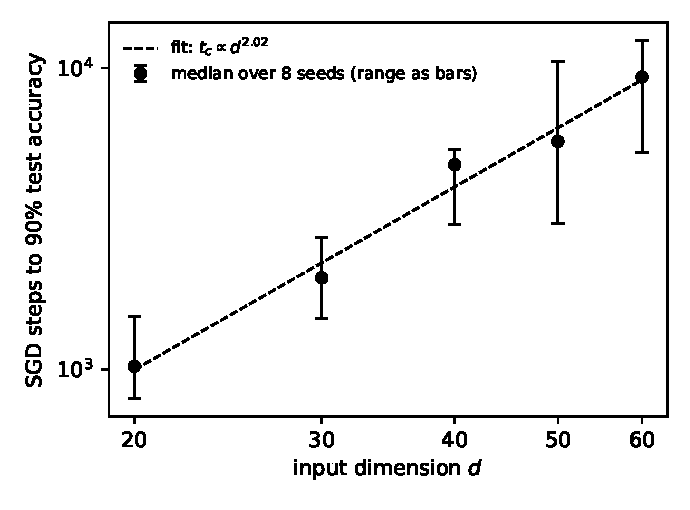
\includegraphics[width=0.62\linewidth]{../figures/parity-scaling.pdf}
\caption{Median SGD steps to \ParityThresh{} test accuracy against input dimension for a
hidden 3-sparse parity, log-log, \ParitySeeds{} seeds per point, bars spanning
the seed range. The fitted exponent \ParitySlope{} is the measured price of the
search in the recipe stated in the text.}
\label{fig:parity}
\end{figure}

What the experiment does and does not show. It shows one recipe's cost growing
as the power law the class floor predicts, in the regime where the recipe's
steps are noisy correlational queries. It does not measure the floor itself,
since no experiment can quantify over algorithms, and it says nothing about
structural adversaries, for which noiseless parity is easy. It is the empirical
face of the no-aiming postulate for the class that trains, and nothing more.


\section{The corpus, mapped onto the framework}
\label{sec:map}

This section places the families the survey covers into
Definition~\ref{def:skeleton}, to show that nothing in the framework is particular
to one of them.

\begin{description}
  \item[Membership inference.] Distinguish. The worlds differ by one record in the
        corpus. The adversary's view is the final model, or black-box access. The
        baseline is the blind attack, which Das et al.\ show beats published
        attacks on eight benchmarks \cite{DZT25}. A shadow-model attack
        \cite{SSSS17,CCNSTT22} is generic and costs $N \cdot T$ steps for $N$ shadow
        models. The verifier of Zhang et al., who cannot sample the null hypothesis
        because doing so ``would require training new large models''
        \cite{ZDKT25}, is an auditor with a read budget of zero steps.
  \item[Membership inference from gradients.] Distinguish, with the adversary's
        view set to gradients, Example~\ref{ex:views}. Fact~\ref{fact:determine}
        says which lossy view the scenario must name.
  \item[Gradient inversion.] Produce. The view is gradients or activations at a
        port, and the criterion is reconstruction within a tolerance. The
        reconstruction-robustness definition of Balle, Cherubin and Hayes already
        supplies the criterion and the oblivious baseline \cite{BCH22}, and the
        gradient-inversion literature, for instance \cite{BDJV22}, supplies
        attacks with no stated criterion. Passive observation of a federated round
        is a read-only attachment. A malicious server is a write.
  \item[Computational differential privacy.] Distinguish, with the worlds drawn by
        the challenger as neighbouring corpora and the distinguisher bounded
        \cite{MPRV09}. Recipe noise, Section~\ref{sec:view}, is where the mechanism
        lives.
  \item[Evasion.] Produce. The criterion is a label change inside a ball around a
        given input. The baseline is random noise in the same ball, which the
        concentration results show already succeeds on some tasks
        \cite{GMFSRWG18}. Access is a view: black-box is the metered wrapper,
        white-box is the final model, and transfer is a shadow model plus the
        adversary's own gradient computation. The number of gradient steps an
        attack is allowed, which the evaluation guidance of Carlini et al.\ declines
        to bound \cite{CAPBRTGMK19} and which Suya et al.\ use to rank attacks
        \cite{SSZHTE24}, is the adversary's running time in
        Definition~\ref{def:generic}.
  \item[Extraction.] Produce. The games of \texttt{games.tex} are this case with
        the view set to black-box access, and their two-party pricing is
        Section~\ref{sec:cost}.
  \item[Poisoning.] A write budget at the corpus. Availability poisoning is
        produce, with the criterion an accuracy drop. Certified defences bound the
        drop for every write within the budget \cite{SKL17}. Robust estimation in
        high dimensions is the case where the defender is polynomial time and the
        writer is unbounded except in the fraction it may change
        \cite{DKKLMS16}.
  \item[Proof-of-learning.] Produce. The criterion is a trace that a verifier
        accepts. The honest prover's trace comes from $T$ oracle steps, and forging
        is producing an accepted trace in fewer. Jia et al.\ require that forging
        cost at least as much as honest training and conjecture rather than prove
        it \cite{JYCDTCP21}. In this framework the requirement is a bound on the
        forger's steps relative to $T$, and the attacks that break their scheme
        \cite{FJTYCDCP23} are generic or structural according to whether they call
        the oracle.
  \item[Watermarking.] Distinguish, with a secret as the hinge: the detector holds
        the key and the distinguisher does not, as in Christ, Gunn and Zamir
        \cite{CGZ23}.
  \item[Filtering and auditing.] Distinguish, where the designated party is an
        auditor whose read budget is stated relative to the model's own cost.
\end{description}

\section{The backdoor game, as far as it is fixed}
\label{sec:backdoor}

This is the one game that composes both criteria. It is stated here to the extent
it has been agreed, with the open decisions marked.

\paragraph{Fixed.} Three roles. A \emph{planter} intervenes during training
through a write budget at a port or at the corpus. An \emph{auditor} observes
through a view and a read budget and outputs a world guess, the distinguish
criterion. An \emph{activator} holds a secret drawn with min-entropy $h$, chosen
by the planter, and tries to elicit a stated behaviour from the final model, the
produce criterion. The activator's baseline is the success of an activator without
the secret, which is the non-replicability property of Goldwasser, Kim,
Vaikuntanathan and Zamir \cite{GKVZ22}. The auditor never holds the secret,
because an auditor given the secret detects by running the activator, so
undetectability is meaningful only against auditors without it.

\paragraph{Fixed.} The planter is generic, Definition~\ref{def:generic}. The
theory constructions in the corpus all give the planter control of training
itself and all place cryptographic structure inside the model. Goldwasser, Kim,
Vaikuntanathan and Zamir achieve black-box undetectability from digital
signatures and white-box undetectability for two specific training paradigms
from continuous LWE and sparse PCA \cite{GKVZ22}. Kalavasis et al.\ achieve
white-box undetectability for pipelines that end in an obfuscation step
\cite{KKOSVZ24}. Draguns et al.\ compile a hash-based digital locker into a
transformer and achieve unelicitability, which they state plainly is not
white-box undetectability \cite{DGMRLW24}. A planter that only writes to the
corpus and faces an honest recipe is the case those constructions do not cover.

\paragraph{Fixed.} The auditor performs detection, not reconstruction. The
question is whether some intervention occurred, and the auditor is not asked to
say which.

\begin{openq}[Non-triviality]
\label{oq:nontrivial}
By Fact~\ref{fact:differ}, a planter whose writes leave the distribution of the
auditor's view unchanged is undetectable and has done nothing. The game needs a
condition on world 1 that rules this out. The activator's success is one such
condition. If the game is to be stated without requiring the backdoor to work at
inference, another condition must replace it, for instance a minimum write budget
together with a declared difference in the label distribution of the written
examples. Which condition to use is not decided.
\end{openq}

\begin{openq}[Where the planter writes]
The planter may write at the corpus, at a training port, or by replacing the data
distribution itself. These give different games, and the last puts no fraction
in the game at all. Which of them the survey's backdoor section treats first is not
decided.
\end{openq}

The corpus-level half of the game's first theorem is a specialization of
existing machinery, and it is worth stating because it prices a party this
literature leaves unpriced.

\begin{proposition}[Undetectability against a query-bounded corpus auditor]
\label{prop:sda}
Fix the backdoor game in which world 0 draws the corpus from a distribution
$D_0$ and world 1 draws it from a distribution the planter selects out of a
family $\mathcal{S}$, and grant the auditor, as its view of the data, a
$\mathrm{VSTAT}(m)$ interface to the corpus distribution with a query budget.
This is the decision problem between $D_0$ and $\mathcal{S}$ in the statistical
algorithms model, and the statistical-dimension lower bound of Feldman et al.\
prices it: an auditor with fewer queries than the statistical dimension at the
matching discrimination parameter fails to decide the world at their stated
success level \cite{FGRVX17}. In their planted bipartite $k$-clique
instantiation, on graphs of size $N$ with $k \le N^{1/2-\delta}$ for constant
$\delta > 0$: deciding requires $N^{\Omega(\log r)}$ queries to
$\mathrm{VSTAT}(N^2/(r k^2))$ for every $r > 0$, and in particular
$N^{\Omega(\log N)}$ queries to $\mathrm{VSTAT}(N^{2-\delta}/k^2)$.
\end{proposition}

\begin{proof}
Specialization. The auditor's task, as fixed, is the model and the problem of
Feldman et al., and the parameters are their Theorem 2.9 \cite{FGRVX17}. Nothing
beyond the specialization is claimed.
\end{proof}

Four boundaries keep the proposition honest. The $\mathrm{VSTAT}(m)$ interface
is an oracle to the population distribution whose answer tolerance models the
averages of roughly $m$ independent samples, which is how Feldman et al.\
motivate it, so the correspondence to an auditor holding a corpus of about $m$
records is the model's own reading and not a theorem. It prices an auditor whose
access to the data is statistical averages, and says nothing about an auditor
who reads individual records, for whom the raw-sample view makes the problem
different. It does not touch the auditor who views the trained model rather than
the corpus, and that transfer is open. And it does not assert that a generic
planter can meet a non-triviality condition with a clique-shaped poison, which
is Open~\ref{oq:nontrivial}. The proposition instantiates the
distribution-replacement variant of the planter, the third option of the open
question on where the planter writes, and its floor comes entirely from the view
restriction, which is the division of labour Section~\ref{sec:passive} states.

\begin{openq}[The model-level auditor]
Whether Proposition~\ref{prop:sda} transfers to an auditor viewing the final
model, rather than the corpus, is not known, and it is the half of the first
theorem that would price backdoor detection as deployed defences practice it.
\end{openq}

\section{What is deferred, and what remains open about the oracle}

\begin{deferred}[The criterion for generation]
The produce criterion assumes a predicate the challenger can evaluate. For a
language model asked to be harmless, the predicate is not something we can write
down. Villa et al.\ idealize that predicate as a ground truth and bound the gap to a
computable judge \cite{VDKMR26}. This framework does not yet include that second
idealization, and a game about generation needs it.
\end{deferred}

\begin{deferred}[Classification]
The tolerance in a produce criterion assumes a metric on outputs. For classifiers
under the zero-one metric, the propositions in \texttt{games.tex} that rest on a
Lipschitz constant do not apply, and the produce games need a separate treatment.
\end{deferred}

\begin{openq}[Declaration]
Section~\ref{sec:class} fixes that what the adversary may exploit is what the game
declares about the recipe's output. The framework does not yet say what a
declaration may contain. Too little, and every theorem is about random functions.
Too much, and the declaration is the theory of learning the oracle was introduced
to avoid. The declaration must also assert that the recipe has no known shortcut,
because the postulates are false where one exists: a convex recipe such as linear
regression has a closed-form endpoint, so the content of its trace is obtainable
with none of its steps. The idealization is only credible for recipe classes in
the no-known-shortcut regime, as the random oracle model is only credible for hash
functions with no known structure. Where that line sits is the main open question
about the oracle itself.
\end{openq}

\begin{openq}[Uninstantiability]
Random-oracle proofs are known to have instantiations for which the proved
theorem fails, by the construction of Canetti, Goldreich and Halevi \cite{CGH04}.
Whether the analogous phenomenon arises when the learning oracle is replaced by a
concrete recipe is not known. A learning analogue of their diagonalization, a game
secure in this model that every concrete recipe implements insecurely, would put
the same known bound on this methodology that theirs put on the random oracle.
\end{openq}

\bibliographystyle{plain}
\bibliography{../refs}

\end{document}
